\section{Implementation} \label{sec:implementation}
% Tobias

% Forward / Backward engineering
When creating the database we used forward engineering to auto generate the 
database from a MySQL EER diagram. The diagram can be seen in 
Figure~\ref{fig:EER}. This had the advantage that the EER diagram could easily 
be made as a translation of the ER Diagram described in 
Section~\ref{sec:design}. This means that it was relatively easy to 
implementation the database, in accordance with the design. We only had to make 
sure that our translation from the ER diagram to the MySQL EER diagram was 
correct to guarantee that the implemented database worked as desired. However, 
this proved more difficult than expected. Because although it could be directly 
translated, it did happen that the way we actually wanted to implement it, was 
not strictly in accordance with the translation of the design. This sometimes 
resulted in changes of the design, as we realized the design was not in 
accordance with the desired functionality. Other times the desired effect was 
achieved although not in accordance with the translation. This can be seen in 
the weak relations \emph{from} and \emph{to} in which the entity \emph{Track} 
has total participation. In order to ensure the total participation, 
\emph{from} and \emph{to} could be primary keys in the entity \emph{Track}. But 
since we wanted to allow having multiple parallel tracks, we made the attribute 
\emph{Id} the primary key. Obviously, we could have made a combined primary 
key, from all three attributes, but this would have allowed for duplicate Ids, 
which we were not interested in. We therefore kept the Id as the primary key, 
and ensured the existence of \emph{from} and \emph{to} by disallowing them from 
having the special value \emph{null}.

\subsection{MySQL EER Diagram}

As described above the EER diagram, seen in Figure~\ref{fig:EER}, was made from 
the hand drawn Entity Relation Diagram show in Figure~\ref{fig:ER}.

Although the EER diagram only is a model and not a database itself. The diagram 
representation is so precise a description of the database, that the database 
can be created from it (known as forward engineering). Likewise the databases 
can be backward engineered into diagrams, which can be a great help, when 
trying to understand an existing database. In this project forward engineering 
on the MySQL EER diagram was used to generate the SQL file shown in 
Appendix~\ref{app:db}. This single file, when run, creates the entire database 
exactly as described by the digram. However, the database is empty and has no 
functionality. There is one thing, that could not be easily transferred from the hand drawn ER diagram to the MySQL EER Diagram. And that is the total participation between \emph{Route} and \emph{RouteTracks}, as described in the design section. There is no innate way to detect if \emph{Route} has any tracks stored in \emph{RouteTracks}. So implementing the total participation relationship would result in lackluster and suboptimal solutions.

The population and common manipulation of the database is 
described in Section~\ref{sec:prog}

\begin{figure}
    \centering
    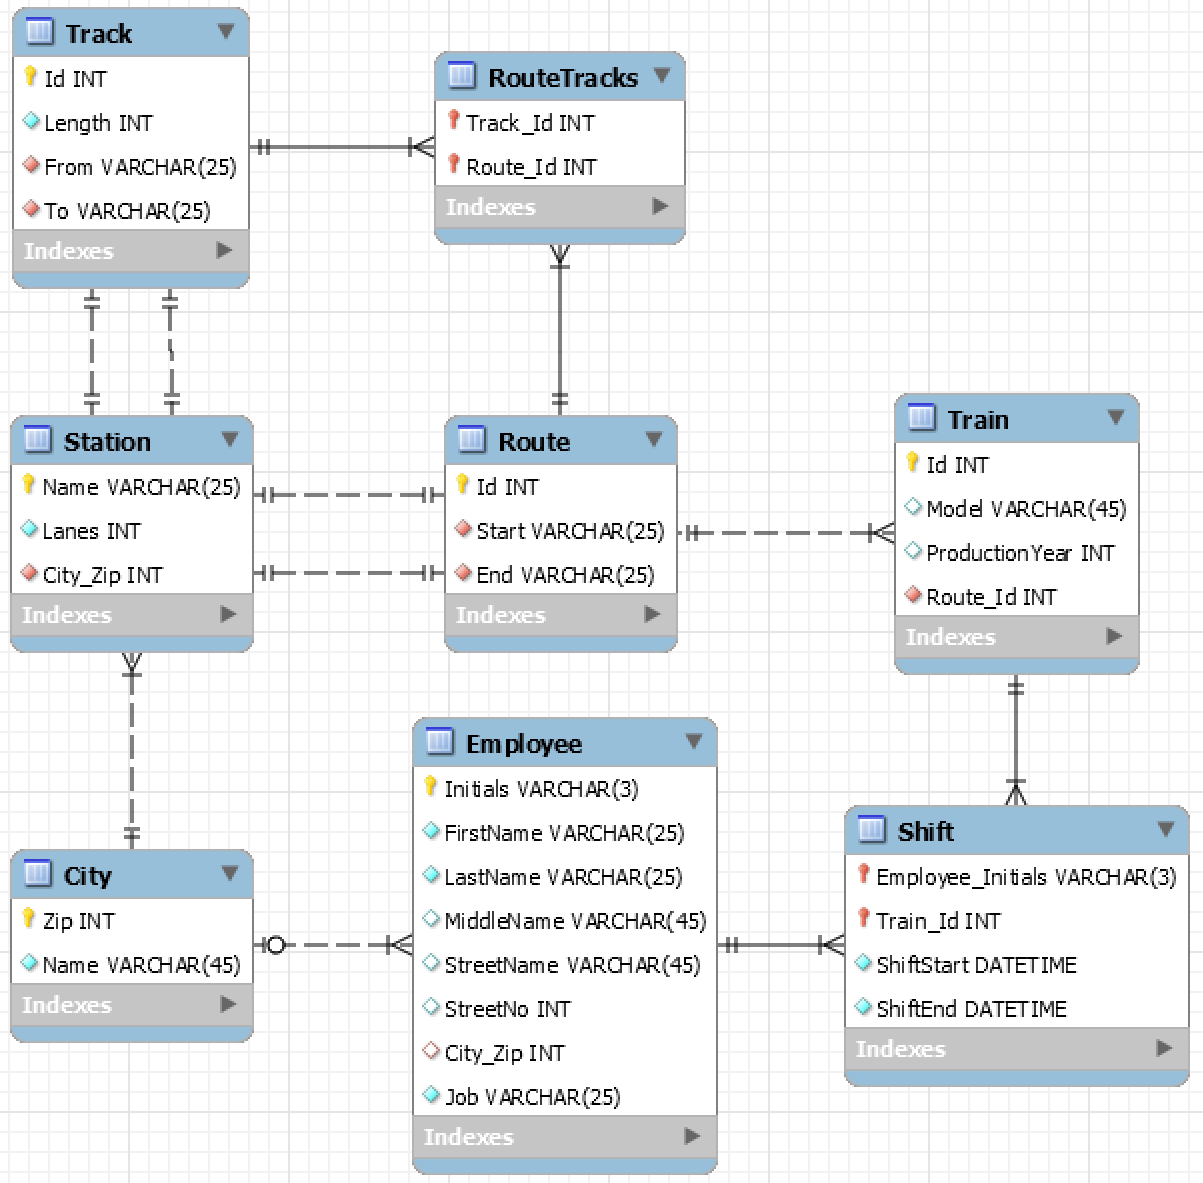
\includegraphics[width=\textwidth]{img/EER.png}
    \caption{EER Diagram implemented in MySQL}
    \label{fig:EER}
\end{figure}

\subsection{Normalization}
% Include this section if the database does not conform to the 3'rd normal form
% Section describes how 3'rd normal form was achieved
This section deals with the normalization of all tables in the database. In 
particular whether it is in conformance with the first, second, and third 
normal forms, and if not, how the normalizations were achieved. It is important 
to note that the normalisations were obtained throughout the process and not as 
a single step near the end. The steps towards each normalisation may therefore 
not have taken part in order, and some normalisations were performed on early 
stages of the database, that are not covered in this report, as changes 
happened rapidly. 

\subsubsection{First Normal Form}
For at table to be in first normal form, the following is required:
\begin{itemize}
    \item Each cell in the table has a single value, i.e., elements are atomic!
    \item All entries in a column have values from the same domain
    \item Each column has a unique name
    \item Each row has a unique Primary Key
    \item The order of the rows does not matter
    \item The order of the columns does not matter
    \item A single attribute must not be sequenced into multiple columns
\end{itemize}
All but the last one are taken care of by MySQL, as it is not possible to 
generate a table that does not obey by the first five rules. However, it is 
entirely up to the database engineers to ensure the last requirement is upheld. 
And from looking at the EER diagram, it might seem that the foreign keys 
\emph{start} and \emph{stop} in the entity \emph{Route}, might violate the 
restriction, and thus that the table is not even normalized to the first normal 
form. However, although the two attributes are much alike, they are not a 
sequence of the same attribute. As matter of fact such a sequence does exist, 
but is stored through the \emph{Track} and \emph{RouteTrack} relations, exactly 
to ensure the table conforms to the first normal form. 

\subsubsection{Second Normal Form}
For a table to be in second normal form, it must be in first normal form and 
every single one of its non primary key attributes must depend on the primary 
key. This seems trivial as without even without putting any effort into it, our 
database was in the second normal form. This is because when generating the 
database it seems natural to only associate attributes within the entities, 
they belong to, working this way the attributes more or less automatically 
depend on the primary key (assuming the primary key is selected reasonably). 

\subsubsection{Third Normal Form}
For a table to be in third normal form, it must be in second normal form and 
there cannot be any transitive attribute dependencies. That is to say that even 
though two attributes both depend on the primary key, if one can be derived 
from the other, the table is not in third normal form. This was initially the 
case as the employees originally had both a \emph{city} and a \emph{zip code} 
associated with them, as part of their address. Clearly both depends on the 
person, as they describes (part of) his address. But one can be derived from 
the other, so in order to obtain the third normal form the \emph{City} entity 
was created, so that each pair of zip codes and city names would only be stored 
once.

